\documentclass{article}
\usepackage[utf8]{inputenc}

\usepackage{tikz}
\usepackage{tikz-cd}
\usepackage{graphicx} % Required for inserting images
\usepackage[a4paper, margin=1in]{geometry}
\usepackage{amsfonts}
\usepackage{amsmath} % Set custom margins
\usepackage{parskip}
\usepackage{amssymb} % disable indentation
\usepackage{amsthm}


\title{Category Theory - Lecture 2 (Notes)}
\author{Vorashil Farzaliyev}
\date{September 2024}

% Define a new theorem style that starts content on a new line


\newtheorem{remark}{Remark}[section]
\newtheorem{lemma}{Lemma}[section]
\newtheorem{proposition}{Proposition}[section]
\newtheorem{definition}{Definition}[section]
\newtheorem{observation}{Observation}[section]
\newtheorem{example}{Example}[section]
\newtheorem{theorem}{Theorem}[section]
\newtheorem{note}{Note}[section]


\begin{document}
    \maketitle


    \section{Examples of categories - Posets}

    Let $(P, \leq)$ be a poset.
    \begin{itemize}
        \item $a \leq a$ for all $a \in P$.
        \item $a \leq b$ and $b \leq c$ implies $a \leq c$.
        \item $a \leq b$ and $b \leq a$ implies $a = b$.
    \end{itemize}
    For example,

    \[
        P =
        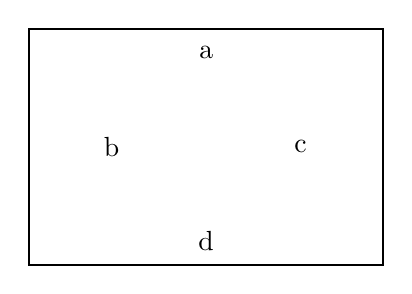
\begin{tikzpicture}
            [baseline={(current bounding box.center)}, scale=1.5]
            % Draw the rectangle
            \draw[thick] (0,0) rectangle (3,2);

            % Place the points
            \node at (1.5, 1.8) {a};  % Top point
            \node at (0.7, 1) {b};     % Middle left point
            \node at (2.3, 1) {c};     % Middle right point
            \node at (1.5, 0.2) {d};  % Bottom point
        \end{tikzpicture}
        \quad \text{where } a \geq b, \; a \geq c, \; b \geq c, \; c \geq d.
    \]

    \begin{definition}[Category of posets]
        Let $\underline{P}$ be a category.
        \begin{itemize}
            \item $\text{Ob}(\underline{P}) = P$
            \item $\forall a, b \in P$
            \[
                \underline{P}(a, b) =
                \begin{cases}
                    \{*\} & \text{if } a \leq b, \\
                    \emptyset & \text{otherwise}.
                \end{cases}
            \]
        \end{itemize}
        with the following axioms satisfied:
        \begin{itemize}
            \item \textbf{Associativity}:
            \[
                \underline{P}(b,c)\times \underline{P}(a,b) \to \underline{P}(a,c)
            \]
            \item \textbf{Identity}:
            \[
                I_a \in \underline{P}(a,a) \ \text{ by reflexivity}
            \]
        \end{itemize}
    \end{definition}

    We can see how multiplication is associative and identity is reflexive.

    \[
        P =
        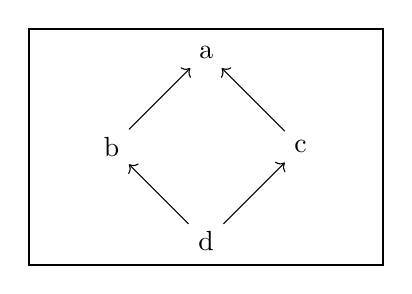
\begin{tikzpicture}
            [baseline={(current bounding box.center)}, scale=1.5]
            % Draw the rectangle
            \draw[thick] (0,0) rectangle (3,2);

            % Place the points
            \node (A) at (1.5, 1.8) {a};  % Top point
            \node (B) at (0.7, 1) {b};    % Middle left point
            \node (C) at (2.3, 1) {c};    % Middle right point
            \node (D) at (1.5, 0.2) {d};  % Bottom point

            % Draw arrows
            \draw[->] (D) -- (B);  % Arrow from d to b
            \draw[->] (D) -- (C);  % Arrow from d to c
            \draw[->] (B) -- (A);  % Arrow from b to a
            \draw[->] (C) -- (A);  % Arrow from c to a
        \end{tikzpicture}
        \quad \text{where } a \geq b, \; a \geq c, \; b \geq c, \; c \geq d.
    \]


    \newpage


    \begin{note}[Size Issue]
        \newline
        \\

        \begin{itemize}
            \item By Russel's paradox, there is no set of all sets.
            So we need to phrase the definition of category catefully.
            \item \textit{For us}, a category has a class of objects, and for any two objects, a class of maps between them
        \end{itemize}
    \end{note}

    \vspace{0.2in}

    \begin{definition}[Locally Small category]
        We say that category $\mathcal{C}$ is a \textbf{locally small} if for any two objects $A, B \in \text{Ob}(\mathcal{C})$,
        the class of maps $\mathcal{C}(A, B)$ is a set.
    \end{definition}

    \vspace{0.2in}


    \begin{definition}[Small category]
        We say that category $\mathcal{C}$ is a \textbf{small} if it's locally small and the class of objects $Ob(\mathcal{C})$ is a set.
    \end{definition}

    \vspace{0.2in}

    \begin{example}
        Let's look at some examples of categories.

        \begin{itemize}
            \item Locally small but not small: $\underline{Set}$, $\underline{Grp}$, $\underline{Top}$
            \item Small: $\Sigma(G), \underline{P}$
        \end{itemize}
    \end{example}


    \section{Isomorphisms}

    \begin{note}
        All isomorphisms in Maths is special case of isomorphisms in Category Theory.
    \end{note}

    \begin{definition}[Isomorphism]
        Let $\mathcal{C}$ be a category.

        \\

        We say that $f: A \to B$ is an \textbf{isomorphism} in $\mathcal{C}$ if there exists a map
        $g: B \to A$ such that
        \[
            \begin{array}{c c} % Create a 2x2 array
                % First commutative diagram in the first column
                \begin{tikzcd}[column sep=4em, row sep=4em]
                    A  \arrow[r, "f"] \arrow[dr, bend right, "1_A"]
                    & B  \arrow[d, "g"]\\
                    & A
                \end{tikzcd}
                &
                % Second commutative diagram in the second column
                \begin{tikzcd}[column sep=4em, row sep=4em]
                    B  \arrow[r, "g"] \arrow[dr, bend right, "1_B"]
                    & A  \arrow[d, "f"]\\
                    & B
                \end{tikzcd} \\
                % Text underneath each diagram
                \text{$1_A = gf$} & \text{$1_B = fg$}
            \end{array}
        \]

        We call $g$ the \textbf{inverse} of $f$.
    \end{definition}

    \subsection{Examples}

    \begin{itemize}
        \item In \underline{Set theory}: isomorphisms are bijections.
        \item In \underline{Group theory}: isomorphisms are group homomorphisms.
        \item In $\underline{Topology}$: isomorphisms are continuous functions.
        \item In $\Sigma(G)$:
        \[
            \begin{tikzcd}[scale=4.5]
                * \arrow[loop left, "f"] \arrow[loop right, "g"] \arrow[loop above, "h"]
            \end{tikzcd}
        \]
        \item In $\underline{P}$:
        \[
            \begin{tikzcd}[column sep=4em, row sep=4em]
                A \arrow[r, bend left=50, "\leq"]
                & B \arrow[l, bend left=50, "\leq"]
            \end{tikzcd} \Leftrightarrow a = b
        \]
        Identities are always isomorphisms.
    \end{itemize}

    \subsection{Uniquness of inverses}

    \begin{proposition}
        Let $f: A \to B$ be a map in a category $\mathcal{C}$. If the inverse of $f$ exists, then it is unique.
    \end{proposition}

    \begin{proof}
        Let $g_1, g_2: B \to A$ be inverses of $f$.

        We claim that $g_1 = g_2$.

        \begin{itemize}
            \item $g_1:$
            \[
                g_1 f = 1_A \quad \text{and} \quad f g_1 = 1_B
            \]
            \item $g_2:$
            \[
                g_2 f = 1_A \quad \text{and} \quad f g_2 = 1_B
            \]
        \end{itemize}

        We can write
        \[
            \begin{array}{c c} % Create a 2x2 array
                % First commutative diagram in the first column
                \begin{tikzcd}[column sep=4em, row sep=4em]
                    A  \arrow[r, "f"] \arrow[dr, bend right, "1_A"]
                    & B  \arrow[d, "g_1 \text{ or } g_2"]\\
                    & A
                \end{tikzcd}
                &
                % Second commutative diagram in the second column
                \begin{tikzcd}[column sep=4em, row sep=4em]
                    B  \arrow[r, "g_1 \text{ or } g_2"] \arrow[dr, bend right, "1_B"]
                    & A  \arrow[d, "f"]\\
                    & B
                \end{tikzcd} \\
                % Text underneath each diagram
            \end{array}
        \]

        That is
        \[
            \begin{tikzcd}[column sep=7em, row sep=2em]
                & B \arrow[dr, "g_1"]  \\
                B \arrow[ur,  "1_B"] \arrow[dr, "g_2"] \arrow[rr, bend left = 95, "g_1"] \arrow[rr, bend right=95, "g_2"] & & A\\
                & A \arrow[ur, "1_A"] \arrow[uu, "f"]
            \end{tikzcd} \quad
            \Leftrightarrow \quad
            \begin{tikzcd}[column sep=7em, row sep=2em]
                B\arrow[bend left, "g_1"]{r}\arrow[bend right, "g_2"]{r}&A
            \end{tikzcd}
        \]

        Using this diagram, we can write
        \[
            \begin{align}
                g_1 &= g_1 \ 1_B \quad \text{by axiom of identity} \\
                &= g_1 \ f \  g_2  \quad \text{since } f \ g_2 = 1_B \\
                &= 1_A \ g_2 \quad \text{since } g_1 \ f = 1_A \\
                &= g_2 \ 1_B \quad \text{by axiom of identity} \\
                &= g_2
            \end{align}
        \]
    \end{proof}

    \begin{note}
        When $f: A \to B$ has an inverse, we can write $f^{-1}: B \to A$ for the inverse.
    \end{note}

    \subsection{Terminal and Initial objects}

    \begin{definition}[Terminal object]
        Let $\mathcal{C}$ be a category.

        An object $T$ of $\mathcal{C}$ is a \textbf{terminal object} if for any object $A \in \text{Ob}(\mathcal{C})$, there exists a unique map $A \to T$.
    \end{definition}

    \begin{definition}[Initial object]
        Let $\mathcal{C}$ be a category.

        An object $I$ of $\mathcal{C}$ is \textbf{initial} if for any object $A \in \text{Ob}(\mathcal{C})$, there exists a unique map $f: I \to A$.
    \end{definition}

    \subsubsection{Examples}
    \begin{itemize}
        \item In \underline{Set}, the terminal object is $\{*\}$.
        \item In \underline{Grp}, the terminal object is $\{*\}$.
        \item In \underline{P}, the following proposition is true.
    \end{itemize}

    \vspace{0.2in}

    \begin{proposition}
        Let $\mathcal{C}$ be a category.

        If  $T$ and $T'$ are terminal objects of $\mathcal{C}$, then $T$ and $T'$ are isomorphic.
    \end{proposition}

    \vspace{0.2in}

    \begin{proof}
        Let $f: T \to T'$ be the unique map from $T$ to $T'$.

        \[
            \begin{array}{c c} % Create a 2x2 array
                % First commutative diagram in the first column
                \begin{tikzcd}[column sep=4em, row sep=4em]
                    T  \arrow[r] \arrow[dr, bend right, "1_{T}"]
                    & T'  \arrow[d]\\
                    & T
                \end{tikzcd}
                &
                % Second commutative diagram in the second column
                \begin{tikzcd}[column sep=4em, row sep=4em]
                    T'  \arrow[r] \arrow[dr, bend right, "1_{T'}"]
                    & T  \arrow[d]\\
                    & T'
                \end{tikzcd} \\
                % Text underneath each diagram
            \end{array}
        \]
    \end{proof}

\end{document}
